\chapter{A complete target-specific scientific workflow}\label{workflow:suite}

The pairwise algebraic engine answers whether two mechanisms can be separated. Many experiments involve several plausible mechanisms, some of which agree on the property of interest. Reconstructing every mechanism would then solve a harder problem than the scientific question requires. This chapter closes that interface with a finite-family design and inference procedure.

\section{Compatible models are the common output}
Let $\Theta$ be a model family and $g:\Theta\to\mathcal G$ the target. A data-dependent set $C_t\subseteq\Theta$ contains the mechanisms still compatible with the accessible evidence at time $t$. Define the retained target set
\[
 T_t=g(C_t).
\]
A scalar target gives an interval or a more general subset of the real line; a discrete scientific question gives a set of labels. The output need not identify a single mechanism.

\begin{theorem}[Target and resource composition]\label{workflow:composition}
Suppose a fixed true mechanism $\theta_*$ belongs to the declared family. Let $G$ be a joint calibration event with $P(G^c)\le\delta$. Suppose
\[
 P\{G\ \text{and}\ \theta_*\notin C_t\ \text{for some }t\}\le\alpha.
\]
An output made only when it is valid for every target in the nonempty set $g(C_t)$ is invalid at some time with probability at most $\alpha+\delta$. If a resource certificate additionally gives $P\{G\text{ and }W>B\}\le\beta$, then the probability of any invalid output or expenditure above $B$ is at most $\alpha+\beta+\delta$.
\end{theorem}
\begin{proof}
On $G$, if $\theta_*\in C_t$, then $g(\theta_*)\in g(C_t)$ and every output valid for that whole set is valid for the actual target. Thus an invalid output on $G$ implies the coverage failure in the premise. The first assertion follows by adding $P(G^c)$. For the second, take a union with the resource failure on $G$. Calibration failure is added once. No independence between the data, resource expenditure and calibration event is needed.
\end{proof}
The premise is an unconditional intersection bound. Conditioning an otherwise valid concentration inequality on a favorable calibration event does not automatically supply it. The adequacy chapter gives one construction using predictable tests; externally fixed valid record-law envelopes give another. An empty set triggers abstention, not a vacuous claim that every target has been proved. The theorem composes guarantees but does not establish that the family contains reality.

\section{A finite experiment menu}
Let $H$ be a finite candidate set, with target labels $g(h)$. Each available experiment $e$ has a finite complete record alphabet $\mathcal Y_e$, a nominal law $p_{h,e}$ for every candidate, and a nonnegative selection charge $c_e$. Suppose the actual law under candidate $h$ belongs to the whole-record total-variation ball
\[
 \operatorname{TV}(\widetilde p_{h,e},p_{h,e})\le\eta_{h,e}.
\]
Preparation, measurement backaction, control errors and detector effects must be included in this record-law envelope or separately transferred into it. A bound on an isolated readout probability is not a substitute.

For a pair $i,j$ with different target labels, the event
\[
 A_{ij,e}=\{y:p_{i,e}(y)>p_{j,e}(y)\}
\]
attains the nominal total-variation difference. Its robust separation is
\[
 d_{ij,e}=\operatorname{TV}(p_{i,e},p_{j,e})-\eta_{i,e}-\eta_{j,e}.
\]
If $d_{ij,e}>0$, the declared event probability intervals are disjoint under the two candidates. If the bound is nonpositive, this event does not provide a positive robust separation. Additional structure in the calibration set can support a stronger conclusion than independent TV balls; the present algorithm uses only the stated balls.

A suite $S$ covers the target if every cross-target pair has a positive gap for at least one $e\in S$. Selecting a minimum-charge suite is the finite weighted set-cover problem
\[
 \min_{S\subseteq\mathcal E}\sum_{e\in S}c_e
 \quad\text{subject to}\quad
 \forall i,j:g(i)\ne g(j),\ \exists e\in S:d_{ij,e}>0.
\]
This is established combinatorial optimization. The implementation uses exact dynamic programming on covered pair masks, with explicit pair and state caps. A cap violation is an unsupported-size error, not an impossibility certificate. The objective counts each selected experiment once. Optimizing its repeated execution, elapsed time or full energy is a different problem.

If the menu does not cover the target, the software names the unresolved pairs. This is an obstruction for the declared robust menu. It does not establish that all physically possible experiments fail, nor that the target is unidentifiable under a more precise calibration model.

\section{From the suite to a finite-error target decision}
If every candidate has the same target, no acquisition is needed within that family. Otherwise assign every cross-target pair to one covering experiment. Retain the associated events, merging duplicate events within an experiment, and discard any experiment assigned no pair. Let $L>0$ be the number of retained event tests. For each chosen experiment, choose
\[
 r_e=\frac14\min\{d_{ij,e}:\text{the pair is assigned to }e\}.
\]
The implementation chooses an integer $k$ and record counts $n_e$ satisfying
\[
 \frac{2L}{2^k}\le\alpha,\qquad
 n_e=\left\lceil\frac{k}{2r_e^2}\right\rceil.
\]
These are sufficient, conservative bounds. They use exact rational arithmetic rather than a floating-point logarithm. Since $\exp(1)>2$, Hoeffding's inequality gives
\[
 2\exp(-2n_er_e^2)\le\frac{2}{2^k}.
\]
The nominal laws, events, radii and suite are fixed before the classification records are collected. Within each experiment, the records must be independent and identically distributed under one fixed mechanism. Different experiments need not be mutually independent for the following union bound. If calibration data determine the inputs, the same iid premise must hold conditional on that pre-acquisition information, and the joint calibration event must bound these conditional record laws. Integrating the conditional concentration guarantee then gives the intersection bound on $G$ required by Theorem~\ref{workflow:composition}; conditioning on an arbitrary favorable event is not sufficient.

For each retained event $A$, let $\widehat p_e(A)$ be its frequency. Retain candidate $h$ precisely when, for every retained event,
\[
 |\widehat p_e(A)-p_{h,e}(A)|\le\eta_{h,e}+r_e.
\]

\begin{theorem}[Finite-family target decision]\label{workflow:finiteerror}
Suppose the selected suite covers every cross-target pair and the finite-family and record-law assumptions above hold. With probability at least $1-\alpha$, the retained set contains the fixed true candidate and all retained candidates share its target. Returning that target when the retained set is nonempty, and abstaining when it is empty, has probability at most $\alpha$ of either an incorrect target or an empty retained set. A jointly bounded calibration failure adds once as in Theorem~\ref{workflow:composition}.
\end{theorem}
\begin{proof}
For each event, Hoeffding bounds the difference between empirical frequency and its actual probability by $r_e$ except with probability at most $2/2^k$. The union bound over $L$ events has probability at most $\alpha$. On the complementary event, the actual record-law calibration bound and the triangle inequality retain the true candidate.

For any two retained candidates $i,j$ with different targets, examine their assigned event and experiment. Their nominal event probabilities differ by more than $\eta_{i,e}+\eta_{j,e}+2r_e$, since $d_{ij,e}\ge4r_e>2r_e$. But both candidates' retention would force the difference to be at most that quantity, by applying the triangle inequality through the same empirical frequency. This is a contradiction. Consequently, any nonempty retained set has a single target; on the simultaneous concentration event it is the true target. The failure assertion follows.
\end{proof}
The algorithm cannot recover an erased distinction between mechanisms that share the same target and the same laws. It does not need to do so. Nor does all-rejected abstention prove that a particular alternative model is correct. It identifies a failed inference attempt that warrants checking the contract.

\section{A reproducible five-model example}
Five candidate mechanisms have two target labels, ``even'' and ``odd''. Their binary-record probabilities are:
\begin{center}
\begin{tabular}{lcccc}
\toprule
Model & Target & Left probe & Right probe & Direct probe\\
\midrule
A & even & $1/4$ & $1/4$ & $1/4$\\
A copy & even & $1/4$ & $1/4$ & $1/4$\\
B & even & $3/4$ & $3/4$ & $1/4$\\
C & odd & $1/4$ & $3/4$ & $3/4$\\
D & odd & $3/4$ & $1/4$ & $3/4$\\
\bottomrule
\end{tabular}
\end{center}
A copy is operationally identical to A. The left probe alone leaves A and C unresolved; the right probe alone leaves A and D unresolved. Together they separate every cross-target pair. If the left and right selection charges are one each and the direct probe charge is three, the exact minimum suite is left plus right, with charge two.

\begin{figure}[htbp]
\centering
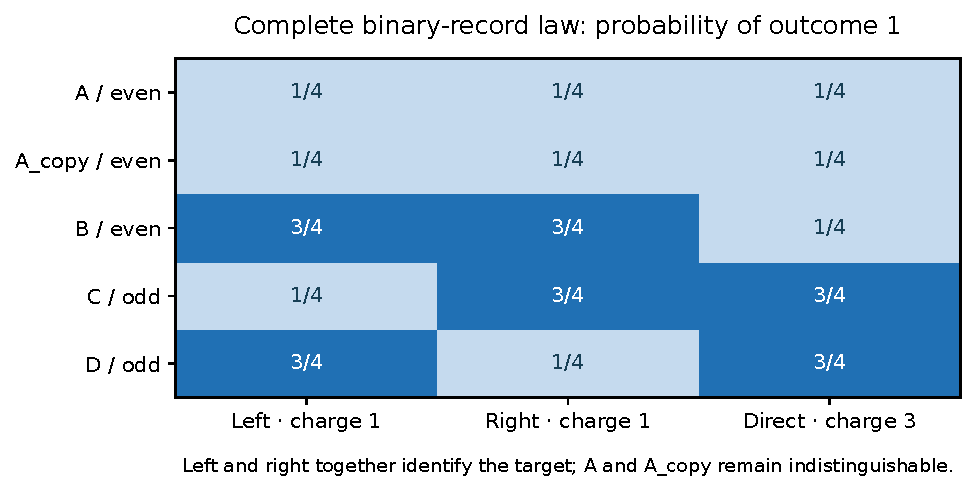
\includegraphics[width=0.88\textwidth]{suite_laws.pdf}
\caption{The complete laws in the finite-menu tutorial. The selected pair of probes resolves the target label while leaving two mechanisms indistinguishable. Every displayed probability is specified analytically.}
\label{workflow:figure}
\end{figure}

Set every whole-record TV radius to $1/100$ and the sampling failure budget to $1/20$. The robust gaps are $12/25$, the selected sampling radii are $3/25$, and the implementation allocates 278 records to each of the two experiments: 556 records in total. Deliberately synthetic frequencies near $1/4$ for both probes retain A and A copy and report ``even''. The complete mechanism remains unidentified. If both TV radii of a pair increase to $1/4$, its nominal half-unit contrast no longer gives positive separation; the robust menu reports the unresolved pairs.

Run the example after installation:
\begin{verbatim}
python examples/suite_tutorial.py --output results/suite_tutorial.json
\end{verbatim}
The JSON includes every nominal law, radius, selected event, record count, retained model and limitation. The supplied counts are synthetic and test the inference interface; they are not simulated discoveries or laboratory measurements.

\section{Using a result in the laboratory}
A useful deployment proceeds through one chain of evidence. First write the physical contract and the target. Then test structural access: either produce an equivalence certificate or generate a candidate experiment. Next verify that calibration leaves a nonzero target-relevant gap. Choose the statistical objective and repetition or feedback policy, and translate the proposed operations into a complete resource ledger. Execute the protocol only after this mapping is justified. Finally retain the models or target values compatible with the actual records, and report abstention or model failure when required.

A result becomes transferable when another group can substitute its calibrated model, run the same checks, execute the returned protocol, and reproduce the promised target coverage or error rate. Different laboratories need not share microscopic mechanisms. They must share the mathematical interface and justify its assumptions for their apparatus.

The next extensions should preserve that standard. Continuous parameter families require validated optimization or analytic envelopes. Large quantum devices require locality, sparsity or other justified structure. Nonstationary experiments require conditional predictions or explicit drift models. Resource comparisons require matched objectives and complete physical accounting. These are clear mathematical and experimental tasks, rather than claims already established by the finite examples.
